%---------------------------------------------------------------------
\begin{frame}{}

    \begin{center}
        \Large \textcolor{maroon}{Decision Making Under Uncertainty (review)}
        \end{center}
\end{frame}
%---------------------------------------------------------------------
\begin{frame}{Poll time}

    Bet:
        \begin{itemize}
            \item 50\% chance of winning \$125
            \item 50\% chance of losing \$100
        \end{itemize}
    $\implies$ Would you take this bet?
    \vspace{5mm}

    \pause
    \textit{\newbold{How to think about it?}}

\end{frame}
%---------------------------------------------------------------------
\begin{frame}{Expected value of this bet}

    Bet:
    \begin{itemize}
        \item 50\% chance of winning \$125
        \item 50\% chance of losing \$100
    \end{itemize}  
    \vspace{5mm}

    \newbold{Expected value (EV)} of the bet:
    \only<1>{
    \begin{equation*}
        EV = Pr(win) \times \text{Amount win} + Pr(lose) \times \text{Amount lose}
    \end{equation*}
    }
    \only<2>{
    \begin{equation*}
        EV = \underbrace{Pr(win)}_{0.5} \times \underbrace{\text{Amount win}}_{\$125} + \underbrace{Pr(lose)}_{0.5} \times \underbrace{\text{Amount lose}}_{-100}
    \end{equation*}
    }
    \only<3>{
    \begin{align*}
        EV &= 0.5 \times 125 + 0.5 \times (-100)\\
        & = 12.5
    \end{align*}
    }
    \only<4>{
        \begin{align*}
            EV &= 0.5 \times 125 + 0.5 \times (-100)\\
            & = 12.5
        \end{align*}
        \vspace{3mm}
        $\implies$ The expected value is positive: \newbold{more-than-fair} bet
    }
\end{frame}
%---------------------------------------------------------------------
\begin{frame}{Expected value vs. expected utility}

    \newbold{Expected value (EV)} of the bet:
    \begin{equation*}
        EV = Pr(win) \times \text{Amount win} + Pr(lose) \times \text{Amount lose}
    \end{equation*}
    \pause
    \vspace{3mm}
    \textit{vs.}\\
    \vspace{3mm}
    \newbold{Expected utility (EU)} of the bet:
    \begin{equation*}
        EU = Pr(win) \times U(\text{Amount win}) + Pr(lose) \times U(\text{Amount lose})
    \end{equation*}
    \pause
    Utility displays behavioral traits: \newbold{risk aversion}\\
    $\implies$ \newbold{How?}

\end{frame}
%---------------------------------------------------------------------
\begin{frame}{Utility: risk-averse}

    \begin{center}

    \begin{tikzpicture}[scale=0.8]
        \begin{axis}[
            width=12.5cm,
            height=8cm,
            axis lines=left,
            xmin=0, xmax=240,
            ymin=0, ymax=16.5,
            xlabel={Wealth, \$},
            ylabel={Utility, $U$},
            xtick=\empty,
            ytick=\empty,
            ticklabel style={font=\scriptsize},
            label style={font=\small},
            clip=false
        ]
        
        % Blue utility curve U(x)=sqrt(x)
        \addplot[
            domain=0:225,
            samples=200,
            very thick,
            blue!70!black
        ] {sqrt(x)};
        
        % Curve label
        \node[
            blue!70!black,
            font=\small,
            yshift=-4pt
        ] at (axis cs:165,14.5) {$U(x)$};
        
        \end{axis}
        \end{tikzpicture}
    \end{center}
    \pause 
    The utility function is \newbold{concave} in income: decreasing marginal utility of income.\\
    Examples: $U(x) = \sqrt{x}$, $U(x) = ln(x)$
\end{frame}
%---------------------------------------------------------------------
\begin{frame}{Utility: risk-neutral}

\begin{center}
    \begin{tikzpicture}[scale=0.8]
        \begin{axis}[
            width=12.5cm,              % adjust for slide size
            height=8cm,
            axis lines=left,
            xmin=0, xmax=240,
            ymin=0, ymax=240,
            xlabel={Wealth, \$},
            ylabel={Utility, $U$},
            xtick=\empty,
            ytick=\empty,
            ticklabel style={font=\scriptsize},
            label style={font=\small},
            clip=false
        ]
        
        % Linear utility curve U(x)=x
        \addplot[
            domain=0:225,
            samples=2,
            very thick,
            blue!70!black
        ] {x};
        
        % Curve label
        \node[
            blue!70!black,
            font=\small,
            yshift=9pt
        ] at (axis cs:197,200) {$U(x)$};
        
        \end{axis}
        \end{tikzpicture}

\end{center}

    \pause 
    The utility function is \newbold{linear} in income.\\
    Example: $U(x) = x$.
\end{frame}
%---------------------------------------------------------------------
\begin{frame}{Utility: risk-loving}

\begin{center}
    \begin{tikzpicture}[scale=0.8]
        \begin{axis}[
            width=12.5cm,
            height=8cm,
            axis lines=left,
            xmin=0, xmax=15,
            ymin=0, ymax=225,
            xlabel={Wealth, $x$},
            ylabel={Utility, $U$},
            xtick=\empty,
            ytick=\empty,
            ticklabel style={font=\scriptsize},
            label style={font=\small},
            clip=false
        ]
        
        % Convex utility curve U(x)=x^2 for x>0
        \addplot[
            domain=0:15,
            samples=200,
            very thick,
            blue!70!black
        ] {x^2};
        
        % Curve label
        \node[
            blue!70!black,
            font=\small,
            yshift=-4pt
        ] at (axis cs:12,180) {$U(x)$};
        
        \end{axis}
        \end{tikzpicture}

\end{center}

    \pause 
    The utility function is \newbold{convex} in income.\\
    Example: $U(x) = x^2$.
\end{frame}
%---------------------------------------------------------------------
\begin{frame}{Back to our bet}

    Bet: 
    \begin{itemize}
        \item 50\% chance of winning \$125
        \item 50\% chance of losing \$100
    \end{itemize}  
    \vspace{5mm}

    Assume:
    \begin{itemize}
        \item You are \newbold{risk-averse} and you know your utility function is $U(x) = \sqrt{x}$
        \item Your initial weath is \$100
    \end{itemize}
    \vspace{3mm}
    \newbold{Expected utility (EU)} of the bet:
    \only<1>{
    \begin{equation*}
        EU = \underbrace{Pr(win)}_{0.5} \times \underbrace{U(\text{Amount win})}_{\sqrt{100 + 125}} + \underbrace{Pr(lose)}_{0.5} \times \underbrace{U(\text{Amount lose})}_{\sqrt{100-100}}
    \end{equation*}
    }
    \only<2>{
    \begin{align*}
        EU &= 0.5 \times 15 + 0.5 \times 0\\
        &= 7.5
    \end{align*}
    }
    \only<3>{
        \begin{align*}
            EU &= 0.5 \times 15 + 0.5 \times 0\\
            &= 7.5
        \end{align*}
    $\implies$ \textit{Are you better off taking the bet?}
    }
\end{frame}
%---------------------------------------------------------------------
\begin{frame}{Are better off taking the bet?}

    \newbold{Expected utility (EU)} of the bet: $EU(\text{bet})=7.5$
    \vspace{5mm}

    What is the utility we would get \textit{without the bet}?
    \begin{align*}
        EU(\text{no bet}) = U(100) &= \sqrt{100}\\
        &= 10 
    \end{align*}
    $\implies$ $EU(\text{bet}) = 7.5 << EU(\text{no bet}) = 10$\\
    $\implies$ It looks like we would be better off \newbold{without taking the bet}!

\end{frame}
%---------------------------------------------------------------------
\begin{frame}{Mapping back to healthcare}

    There are bets or gambles in life we cannot avoid
    \begin{itemize}
        \item Losing a job in a poor economic environment
        \item Getting sick
        \item etc.
    \end{itemize}
    \vspace{5mm}

    We can insure ourselves against this uncertainty $\implies$ \newbold{demand for insurance}

\end{frame}
%---------------------------------------------------------------------
\begin{frame}{}

    \begin{center}
        \Large \textcolor{maroon}{Demand for health insurance}
    \end{center}
\end{frame}
%---------------------------------------------------------------------
\begin{frame}{Back to our bet}

    Bet: 50\% chance of winning \$125, 50\% chance of losing \$100
    \vspace{5mm}

    We have already calculated:
    \begin{itemize}
       \item Expected Value (EV) of the bet \newbold{(it is in USD!)}:
            \begin{align*}
                EV &= Pr(win) \times \text{Amount win} + Pr(lose) \times \text{Amount lose}\\
                &= 12.5 (+100\text{ initial wealth})\\
                &= \$112.5
            \end{align*}
        \item Expected Utility (EU) of the bet \newbold{(it is in utils)}:
            \begin{align*}
                EU &= Pr(win) \times U(\text{Amount win})+ Pr(lose) \times U(\text{Amount lose})\\
                &= 7.5 <<< 10 = U(100)
            \end{align*}
    \end{itemize}
    \pause
    \textit{Let's graph it}!
\end{frame}
%---------------------------------------------------------------------
\begin{frame}{Graphical representation}
    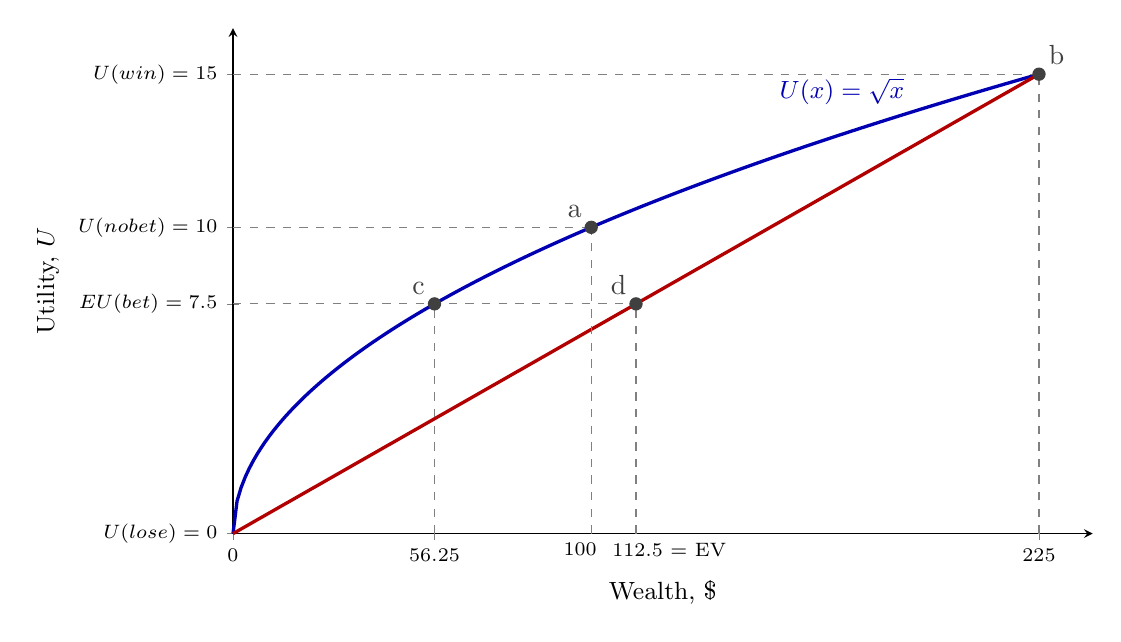
\begin{tikzpicture}
        \begin{axis}[
            width=12.5cm,height=8cm,
            axis lines=left,
            xmin=0,xmax=240,
            ymin=0,ymax=16.5,
            xlabel={Wealth, \$},
            ylabel={Utility, $U$},
            xtick={0,56.25,225},
            ytick={0,7.5,10,15},
            yticklabels={
                {$U(\text{lose})=0$},
                {$EU(\text{bet})=7.5$},
                {$U(\text{no bet})=10$},
                {$U(\text{win})=15$}
            },
            ticklabel style={font=\scriptsize},
            label style={font=\small},
            clip=false
        ]
        
        \node[below, font=\scriptsize, xshift=-4pt] at (axis cs:100,0) {$100$};
        \node[below, font=\scriptsize, xshift=+12pt] at (axis cs:112.5,0) {$112.5$ = EV};

        % Blue utility curve U(x)=sqrt(x)
        \addplot[domain=0:225, samples=200, very thick, blue!70!black] {sqrt(x)};
        
        % Label for the utility curve
        \node[blue!70!black, font=\small, yshift=-4pt]
            at (axis cs:170,14.8) {$U(x)=\sqrt{x}$};
        
        % Red chord from (0,0) to b
        \addplot[very thick, red!70!black] coordinates {(0,0) (225,15)};
        
        % Points a, b, c (dark gray)
        \addplot[only marks, mark=*, mark size=2.2pt, darkgray]
        coordinates {(100,10) (225,15) (112.5,7.5) (56.25,7.5)};
        
        \node[above left,  darkgray] at (axis cs:100,10) {a};
        \node[above right, darkgray] at (axis cs:225,15) {b};
        \node[above left, darkgray] at (axis cs:56.25,7.5) {c};
        \node[above left, darkgray] at (axis cs:112.5,7.5) {d};
        
        % Dashed guides for a
        \draw[dashed, gray] (axis cs:100,0) -- (axis cs:100,10);
        \draw[dashed, gray] (axis cs:0,10) -- (axis cs:100,10);
        
        % Dashed guides for b
        \draw[dashed, gray] (axis cs:225,0) -- (axis cs:225,15);
        \draw[dashed, gray] (axis cs:0,15) -- (axis cs:225,15);
        
        % Dashed guides for c
        \draw[dashed, gray] (axis cs:112.5,0) -- (axis cs:112.5,7.5);
        \draw[dashed, gray] (axis cs:0,7.5) -- (axis cs:112.5,7.5);
        
        % Certainty equivalent (sqrt(56.25)=7.5)
        \draw[dashed, gray] (axis cs:56.25,0) -- (axis cs:56.25,7.5);
        \node[below, font=\scriptsize] at (axis cs:56.25,0) {};
        
        \end{axis}
        \end{tikzpicture}
    
\end{frame}
%---------------------------------------------------------------------
\begin{frame}{Willingness to pay to avoid the bet - certainty equivalent}

    Bet: 50\% chance of winning \$125, 50\% chance of losing \$100
    \vspace{5mm}

    What is the \newbold{certainty equivalent (CE)} of this bet?\\
    \textit{Definition CE: How much money you would rather get for sure rather than taking the bet.}
    \begin{itemize}
        \item If I take the bet, I get utility $EU(\text{bet}) = 7.5$
        \item The certainty equivalent is the amount of money $x$
        that would give me utility 7.5 \textit{for sure}:
        it is $x$ such that $U(x) = 7.5$.
    \end{itemize}
    \pause 
    \vspace{3mm}
    \textit{Let's calculate it!}
\end{frame}
%---------------------------------------------------------------------
\begin{frame}{Willingness to pay to avoid the bet - certainty equivalent}

    Bet: 50\% chance of winning \$125, 50\% chance of losing \$100
    \vspace{5mm}

    What is the \newbold{certainty equivalent (CE)} of this bet?\\
    \vspace{3mm}
    \textit{Let's calculate it!}
    \begin{align*}
        &U(x) = 7.5\\
        \Leftrightarrow &\sqrt{x} = 7.5\\
        \Leftrightarrow &x = 7.5^2\\
        \Leftrightarrow & x = 56.25
    \end{align*}
    $\implies$ The \newbold{certainty equivalent} of this bet is \$56.25.

\end{frame}
%---------------------------------------------------------------------
\begin{frame}{How much would you rather pay to avoid the bet?}

    \newbold{Risk-premium (RP)}: the ``price'' of the insurance contract.\\
    How much would you rather pay to avoid the bet?
    \begin{align*}
        \text{RP} &= EV - CE\\
        &= 112.5 - 56.25\\
        &= 56.25
    \end{align*}

    $\implies$ You would rather pay up to \$56.25 and get utility 7.5 for sure rather than taking the bet!

\end{frame}
%---------------------------------------------------------------------
\begin{frame}{Graphical representation}
    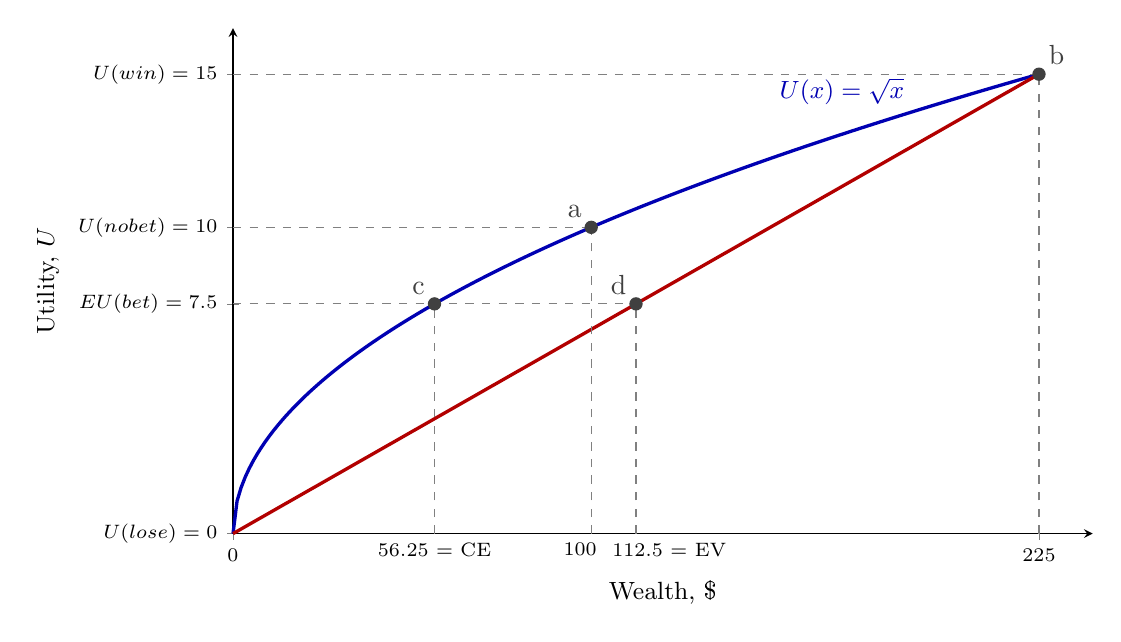
\begin{tikzpicture}
        \begin{axis}[
            width=12.5cm,height=8cm,
            axis lines=left,
            xmin=0,xmax=240,
            ymin=0,ymax=16.5,
            xlabel={Wealth, \$},
            ylabel={Utility, $U$},
            xtick={0,225},
            ytick={0,7.5,10,15},
            yticklabels={
                {$U(\text{lose})=0$},
                {$EU(\text{bet})=7.5$},
                {$U(\text{no bet})=10$},
                {$U(\text{win})=15$}
            },
            ticklabel style={font=\scriptsize},
            label style={font=\small},
            clip=false
        ]
        
        \node[below, font=\scriptsize, xshift=-4pt] at (axis cs:100,0) {$100$};
        \node[below, font=\scriptsize, xshift=+12pt] at (axis cs:112.5,0) {$112.5$ = EV};
        \node[below, font=\scriptsize] at (axis cs:56.25,0) {$56.25$ = CE};

        % Blue utility curve U(x)=sqrt(x)
        \addplot[domain=0:225, samples=200, very thick, blue!70!black] {sqrt(x)};
        
        % Label for the utility curve
        \node[blue!70!black, font=\small, yshift=-4pt]
            at (axis cs:170,14.8) {$U(x)=\sqrt{x}$};
        
        % Red chord from (0,0) to b
        \addplot[very thick, red!70!black] coordinates {(0,0) (225,15)};
        
        % Points a, b, c (dark gray)
        \addplot[only marks, mark=*, mark size=2.2pt, darkgray]
        coordinates {(100,10) (225,15) (112.5,7.5) (56.25,7.5)};
        
        \node[above left,  darkgray] at (axis cs:100,10) {a};
        \node[above right, darkgray] at (axis cs:225,15) {b};
        \node[above left, darkgray] at (axis cs:56.25,7.5) {c};
        \node[above left, darkgray] at (axis cs:112.5,7.5) {d};
        
        % Dashed guides for a
        \draw[dashed, gray] (axis cs:100,0) -- (axis cs:100,10);
        \draw[dashed, gray] (axis cs:0,10) -- (axis cs:100,10);
        
        % Dashed guides for b
        \draw[dashed, gray] (axis cs:225,0) -- (axis cs:225,15);
        \draw[dashed, gray] (axis cs:0,15) -- (axis cs:225,15);
        
        % Dashed guides for c
        \draw[dashed, gray] (axis cs:112.5,0) -- (axis cs:112.5,7.5);
        \draw[dashed, gray] (axis cs:0,7.5) -- (axis cs:112.5,7.5);
        
        % Certainty equivalent (sqrt(56.25)=7.5)
        \draw[dashed, gray] (axis cs:56.25,0) -- (axis cs:56.25,7.5);
        \node[below, font=\scriptsize] at (axis cs:56.25,0) {};
        
        \end{axis}
        \end{tikzpicture}
    
\end{frame}
%---------------------------------------------------------------------
\begin{frame}{Graphical representation}
    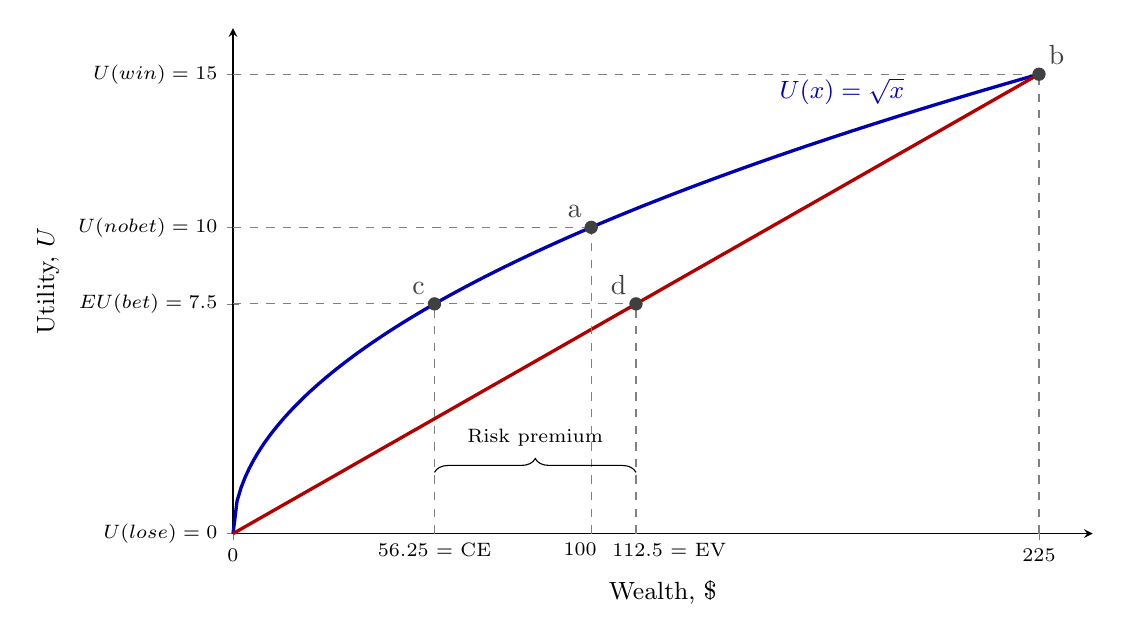
\begin{tikzpicture}
        \begin{axis}[
            width=12.5cm,height=8cm,
            axis lines=left,
            xmin=0,xmax=240,
            ymin=0,ymax=16.5,
            xlabel={Wealth, \$},
            ylabel={Utility, $U$},
            xtick={0,225},
            ytick={0,7.5,10,15},
            yticklabels={
                {$U(\text{lose})=0$},
                {$EU(\text{bet})=7.5$},
                {$U(\text{no bet})=10$},
                {$U(\text{win})=15$}
            },
            ticklabel style={font=\scriptsize},
            label style={font=\small},
            clip=false
        ]
        
        % Manual x labels (shifted)
        \node[below, font=\scriptsize, xshift=-4pt] at (axis cs:100,0) {$100$};
        \node[below, font=\scriptsize, xshift=+12pt] at (axis cs:112.5,0) {$112.5$ = EV};
        \node[below, font=\scriptsize] at (axis cs:56.25,0) {$56.25$ = CE};

        % Blue utility curve U(x)=sqrt(x)
        \addplot[domain=0:225, samples=200, very thick, blue!70!black] {sqrt(x)};
        
        % Utility curve label
        \node[blue!70!black, font=\small, yshift=-4pt]
            at (axis cs:170,14.8) {$U(x)=\sqrt{x}$};
        
        % Red chord from (0,0) to b
        \addplot[very thick, red!70!black] coordinates {(0,0) (225,15)};
        
        % Points a, b, c, d
        \addplot[only marks, mark=*, mark size=2.2pt, darkgray]
        coordinates {(100,10) (225,15) (56.25,7.5) (112.5,7.5)};
        
        \node[above left,  darkgray] at (axis cs:100,10) {a};
        \node[above right, darkgray] at (axis cs:225,15) {b};
        \node[above left,  darkgray] at (axis cs:56.25,7.5) {c};
        \node[above left,  darkgray] at (axis cs:112.5,7.5) {d};
        
        % Dashed guides for a
        \draw[dashed, gray] (axis cs:100,0) -- (axis cs:100,10);
        \draw[dashed, gray] (axis cs:0,10) -- (axis cs:100,10);
        
        % Dashed guides for b
        \draw[dashed, gray] (axis cs:225,0) -- (axis cs:225,15);
        \draw[dashed, gray] (axis cs:0,15) -- (axis cs:225,15);
        
        % Dashed guides for d (expected utility)
        \draw[dashed, gray] (axis cs:112.5,0) -- (axis cs:112.5,7.5);
        \draw[dashed, gray] (axis cs:0,7.5) -- (axis cs:112.5,7.5);
        
        % Certainty equivalent
        \draw[dashed, gray] (axis cs:56.25,0) -- (axis cs:56.25,7.5);
        
        % Risk premium brace INSIDE the graph at y = 2
        \draw[
            decorate,
            decoration={brace, amplitude=5pt}
        ]
        (axis cs:56.25,2) -- (axis cs:112.5,2)
        node[midway, above=6pt, font=\scriptsize] {Risk premium};
        
        \end{axis}
        \end{tikzpicture}
    
\end{frame}
%---------------------------------------------------------------------
\begin{frame}{}

    \begin{center}
        \textcolor{maroon}{Now, you have the tools to think about demand for health insurance!}
    \end{center}
\end{frame}
%---------------------------------------------------------------------
\begin{frame}{Willingness-to-pay for health insurance}

    Assume
    \begin{itemize}
        \item Your intial wealth is \$100,000
        \item You are risk-averse with utility function $U(x) = \sqrt{x}$
        \item The probability to be sick is 10\%
        \item If you get sick, medical expenses are \$40,000
    \end{itemize}
    \vspace{8mm}
    $\implies$ How much are you willing to pay for health insuarnce with \textbf{full} coverage?
\end{frame}
%---------------------------------------------------------------------
\begin{frame}{Willingness-to-pay for health insurance}

    Expected value (EV):
    \vspace{15mm}

    Expected utility (EU):
    \vspace{15mm}

    Certainty equivalent (CE):
    \vspace{15mm}

    \newbold{Risk-premium (RP)}:
    \vspace{15mm}
\end{frame}
%---------------------------------------------------------------------
\begin{frame}{Willingness-to-pay for health insurance}

    Expected value (EV):
    {\color{red}
    \begin{align*}
        EV &= Pr(\text{healthy}) \times \text{Wealth healthy} + Pr(\text{sick}) \times \text{Wealth sick}\\
        &= 0.9 \times 100,000 + 0.1 \times (100,000 - 40,000)\\
        &= 96,000
    \end{align*}
    }

    Expected utility (EU):
    \vspace{5mm}

    Certainty equivalent (CE):
    \vspace{5mm}

    Risk-premium (RP):

\end{frame}
%---------------------------------------------------------------------
\begin{frame}{Willingness-to-pay for health insurance}

    Expected value (EV): {\color{red}$EV =\$96,000$}
    \vspace{5mm}

    Expected utility (EU):
    {\color{red}
    \begin{align*}
        EU &= Pr(\text{healthy}) \times U(\text{Wealth healthy}) + Pr(\text{sick}) \times U(\text{Wealth sick})\\
        &= 0.9 \times \sqrt{100,000} + 0.1 \times \sqrt{100,000 - 40,000}\\
        &= 309.10
    \end{align*}
    }

    Certainty equivalent (CE):
    \vspace{5mm}

    Risk-premium (RP):

\end{frame}
%---------------------------------------------------------------------
\begin{frame}{Willingness-to-pay for health insurance}

    Expected value (EV): {\color{red}$EV =\$96,000$}
    \vspace{5mm}

    Expected utility (EU): {\color{red}$EU = 309.10$}
    \vspace{5mm}

    Certainty equivalent (CE):
    {\color{red}
    \begin{align*}
        &U(x) = 309.10\\
        \Leftrightarrow &\sqrt{x} = 309.10\\
        \Leftrightarrow &x = (309.10)^2\\
        \Leftrightarrow & x = 95,481
    \end{align*}
    }

    Risk-premium (RP):

\end{frame}
%---------------------------------------------------------------------
\begin{frame}{Willingness-to-pay for health insurance}

    Expected value (EV): {\color{red}$EV =\$96,000$}
    \vspace{5mm}

    Expected utility (EU): {\color{red}$EU = 309.10$}
    \vspace{5mm}

    Certainty equivalent (CE): {\color{red}$CE = \$95,481$}
    \vspace{5mm}

    Risk-premium (RP):
    {\color{red}
    \begin{align*}
        \text{RP} &= EV - CE\\
        &= 96,000 - 95,481\\
        &= 519
    \end{align*}
    }

\end{frame}
%---------------------------------------------------------------------
\begin{frame}{Willingness-to-pay for health insurance}

    Expected value (EV): {\color{red}$EV =96,000$}
    \vspace{5mm}

    Expected utility (EU): {\color{red}$EU = 309.10$}
    \vspace{5mm}

    Certainty equivalent (CE): {\color{red}$CE = \$95,481$}
    \vspace{5mm}

    Risk-premium (RP): {\color{red}$RP = \$519$}
    \vspace{5mm}

    $\implies$ You would be willing to pay up to \$519 for full health insurance coverage!

\end{frame}
%---------------------------------------------------------------------
\begin{frame}{Willingness-to-pay for health insurance: not full coverage}

    Assume
    \begin{itemize}
        \item Your intial wealth is \$100,000
        \item You are risk-averse with utility function $U(x) = \sqrt{x}$
        \item The probability to be sick is 10\%
        \item If you get sick, medical expenses are \$40,000
    \end{itemize}
    \vspace{8mm}
    $\implies$ How much are you willing to pay for health insurance with \textbf{full} coverage? {\color{red}$\$519$}\\
    $\implies$ What about if not full coverage? \only<2>{\textit{Next class!}}
\end{frame}
%---------------------------------------------------------------------
\begin{frame}{}
    \begin{center}
    \Large \textcolor{maroon}{Wrapping up}
    \end{center}

\end{frame}
%---------------------------------------------------------------------
\begin{frame}{What we covered today}
        \begin{itemize}
        \item Decision making under uncertainty (review)
        \item Demand for insurance\\
        {\small (expected value, expected utility, certainty equivalent, risk-premium)}
    \end{itemize}
\end{frame}
%---------------------------------------------------------------------
\begin{frame}{To next class}
    \begin{itemize}
        \item \newbold{TO DO}
        \begin{enumerate}
            \item Review this class' material $\implies$ \textit{questions on it?}
            \item Review past material $\implies$ \textit{questions on it?}
        \end{enumerate}
        \vspace{5mm}

        \item Program for next class
        \begin{itemize}
            \item Understanding an insurance plan
            \item Comparing health insurance plans
        \end{itemize}
    \end{itemize}
\end{frame}
%---------------------------------------------------------------------